%MIT License
%
%Copyright (c) 2018 Wang Chen and Jinming Xu
%
%Permission is hereby granted, free of charge, to any person obtaining a copy
%of this software and associated documentation files (the "Software"), to deal
%in the Software without restriction, including without limitation the rights
%to use, copy, modify, merge, publish, distribute, sublicense, and/or sell
%copies of the Software, and to permit persons to whom the Software is
%furnished to do so, subject to the following conditions:
%
%The above copyright notice and this permission notice shall be included in all
%copies or substantial portions of the Software.
%
%THE SOFTWARE IS PROVIDED "AS IS", WITHOUT WARRANTY OF ANY KIND, EXPRESS OR
%IMPLIED, INCLUDING BUT NOT LIMITED TO THE WARRANTIES OF MERCHANTABILITY,
%FITNESS FOR A PARTICULAR PURPOSE AND NONINFRINGEMENT. IN NO EVENT SHALL THE
%AUTHORS OR COPYRIGHT HOLDERS BE LIABLE FOR ANY CLAIM, DAMAGES OR OTHER
%LIABILITY, WHETHER IN AN ACTION OF CONTRACT, TORT OR OTHERWISE, ARISING FROM,
%OUT OF OR IN CONNECTION WITH THE SOFTWARE OR THE USE OR OTHER DEALINGS IN THE
%SOFTWARE.
\documentclass[12pt,a4paper,twoside]{Thesis} % Paper size, default font size and one-sided paper

\graphicspath{%
    {./Pictures/}% 
    {Figures/}% 
}

\usepackage[square, numbers, comma, sort&compress]{natbib} % Use the natbib reference package - read up on this to edit the reference style; if you want text (e.g. Smith et al., 2012) for the in-text references (instead of numbers), remove 'numbers' 

\hypersetup{urlcolor=black, colorlinks=true} % Colors hyperlinks in blue - change to black if annoying
\title{\ttitle} % Defines the thesis title - don't touch this

%extra packages
\usepackage{float}
\usepackage[caption=false,font=footnotesize]{subfig}    % mutiple subfigures
% \renewcommand{\thesubfigure}{\Alph{subfigure}}
\usepackage{color,soul}               % highlighting text
\usepackage{enumerate}
% \usepackage{enumitem}
\usepackage{mydefs}
%--------------------------------------------------------------------------------------------

\begin{document}

\frontmatter % Use roman page numbering style (i, ii, iii, iv...) for the pre-content pages

\setstretch{1.3} % Line spacing of 1.3
% Define the page headers using the Fr package and set up for one-sided printing
\fancyhead{}     % Clears all page headers and footers
\rhead{\thepage} % Sets the right side header to show the page number
\lhead{}         % Clears the left side page header

\pagestyle{fancy} % Finally, use the "fancy" page style to implement the FancyHdr headers

%----------------------------------------------------------------------------------------
%	TITLE PAGE
%----------------------------------------------------------------------------------------

\maketitle

% ----------------------------------------------------------------------------------------
% 	DECLARATION PAGE
% ----------------------------------------------------------------------------------------

\thesisdeclare{I hereby certify that the intellectual content of this thesis is the product of my original research work and has not been submitted for a higher degree to any other University or Institution.}

\setcounter{page}{1}   % counting afterwards

% ----------------------------------------------------------------------------------------
% 	ACKNOWLEDGEMENTS
% ----------------------------------------------------------------------------------------

\setstretch{1.3} % Reset the line-spacing to 1.3 for body text (if it has changed)

\acknowledgements{\addtocontents{toc}{\vspace{0.8em}} % Add a gap in the Contents, for aesthetics

I wish to express my greatest gratitude to my advisor.

% \begin{flushright}
% \emph{Jinming Xu, December 2015}
% \end{flushright}
}

%----------------------------------------------------------------------------------------
%	QUOTATION PAGE
%----------------------------------------------------------------------------------------

\pagestyle{empty} % No headers or footers for the following pages
\emph{``If I had one hour to save the world, I would spend 55 minutes defining the problem and only five minutes finding the solution."}

\begin{flushright}
---Einstein, Albert
\end{flushright}
\null\vfill % Add some space to move the quote down the page a bit

\begin{center}
\large{To my dear family}
\end{center}
\vfill\vfill\null % Add some space at the bottom to position the quote just right

\cleardoublepage % Start a new page and make the next page a right-hand (odd-numbered) page, producing a blank page if necessary

%----------------------------------------------------------------------------------------
%	ABSTRACT PAGE
%----------------------------------------------------------------------------------------

\addtotoc{Abstract} % Add the "Abstract" page entry to the Contents

\abstract{\addtocontents{toc}{\vspace{0.8em}}% Add a gap in the Contents, for aesthetics

% 1. The Problem 2. The Issues 3. The Approach 4. The Results 5. The Experiments 6. The Applications

My abstracts

%----------------------------------------------------------------------------------------
%	LIST OF CONTENTS/FIGURES/TABLES PAGES
%----------------------------------------------------------------------------------------

\pagestyle{fancy} % The page style headers have been "empty" all this time, now use the "fancy" headers as defined before to bring them back

\lhead{\sl{Contents}} % Set the left side page header to "Contents"
\tableofcontents % Write out the Table of Contents

\lhead{\sl{List of Figures}} % Set the left side page header to "List of Figures"
\listoffigures % Write out the List of Figures

%\lhead{\sl{List of Tables}} % Set the left side page header to "List of Tables"
%\listoftables % Write out the List of Tables

%----------------------------------------------------------------------------------------
%	ABBREVIATIONS
%----------------------------------------------------------------------------------------

%\clearpage % Start a new page
%
%\setstretch{1.5} % Set the line spacing to 1.5, this makes the following tables easier to read
%
%\lhead{\emph{Abbreviations}} % Set the left side page header to "Abbreviations"
%\listofsymbols{ll} % Include a list of Abbreviations (a table of two columns)
%{
%\textbf{LAH} & \textbf{L}ist \textbf{A}bbreviations \textbf{H}ere \\
%%\textbf{Acronym} & \textbf{W}hat (it) \textbf{S}tands \textbf{F}or \\
%}

%----------------------------------------------------------------------------------------
%	PHYSICAL CONSTANTS/OTHER DEFINITIONS
%----------------------------------------------------------------------------------------

%\clearpage % Start a new page
%
%\lhead{\emph{Physical Constants}} % Set the left side page header to "Physical Constants"
%
%\listofconstants{lrcl} % Include a list of Physical Constants (a four column table)
%{
%Speed of Light & $c$ & $=$ & $2.997\ 924\ 58\times10^{8}\ \mbox{ms}^{-\mbox{s}}$ (exact)\\
%% Constant Name & Symbol & = & Constant Value (with units) \\
%}

%----------------------------------------------------------------------------------------
%	SYMBOLS
%----------------------------------------------------------------------------------------

\cleardoublepage  % Start a new page (no need if the previous page is list of figures)

\lhead{\emph{Symbols and Acronyms}} % Set the left side page header to "Symbols"

\listofnomenclature{ll} % Include a list of Symbols (a three column table)
{
\multicolumn{2}{l}{\LARGE{\textbf{Symbols}}}\\[0.618cm]
$\mathcal{R}^n$                    &the $n$-dimensional Euclidean space\\
$\mathcal{H}$                      &the Euclidean  space\\
$\norm{\cdot}$                     &the 2-norm of a vector or matrix in Euclidean space\\
$\norm{\cdot}_G$                   &the induced norm of a vector in G-space\\
$\norm{\cdot}_E$                   &the induced norm of a vector or matrix in probabilistic space\\ 


$\odot$                            &the Hadamard (component-wise) product\\
$\otimes$                          &the Kronecker product\\
$\innprod{\cdot}{\cdot}$           &the inner product of two vectors\\
$\circ$                            &the composition of functions\\ [0.618cm]


$\nabla f$                    &the gradient vector\\
$\mathcal{C}^k$               &the function with continuous partial derivatives up to $k$ orders\\
% $T_x\mathcal{M}$              &the tangent space of the set $\mathcal{M}$\\
% $x_i$                         &the $i$-th component of a vector $x$\\
$x_{i,k}$                     &the $i$-th component of a vector $x$ at time $k$\\
$\bar{x}$                     &the vector with the average of all components of $x$ as each element\\ 
$\ones$                       &all-ones column vector with proper dimension\\
$\mathcal{C}$                 &the average space, i.e., $span\{{\bf 1}\}$ \\
$\mathcal{C}^\perp$           &the disagreement space, i.e., $span^\perp\{{\bf 1}\}$ \\
% W                             &the weight matrix\\
% L                             &the Laplacian matrix\\
$\Pi_\parallel$               &the projection matrix to the average space $\mathcal{C}$\\
$\Pi_\perp$                   &the projection matrix to the disagreement space $\mathcal{C}^\perp$ \\ 
$O(\cdot)$                    &order of magnitude or ergodic convergence rate (running average)\\ 
$o(\cdot)$                    &non-ergodic convergence rate\\ 
% $O(\cdot)$                    &the ergodic convergence rate stated in terms of the running average\\ 
% $o(\cdot)$                    &the non-ergodic convergence rate stated in terms of $x_k$\\ 



$\mathcal{N}_i$               &the index set of the neighbors of agent $i$ \\ [1cm]

\multicolumn{2}{l}{\LARGE{\textbf{Acronyms}}}\\[0.618cm]
DOP                      & Distributed Optimization Problem\\
EDOP                     & Equivalent Distributed Optimization Problem\\
SDOP                     & Stochastic Distributed Optimization Problem\\
OEP                      & Optimal Exchange Problem\\
OCP                      & Optimal Consensus Problem\\
DOCP                     & Dynamic Optimal Consensus Problem\\[0.618cm]
AugDGM           & Augmented Distributed Gradient Methods\\
AsynDGM          & Asynchronous Distributed Gradient Methods\\
D-ESC            & Distributed Extremum Seeking Control\\
D-SPA            & Distributed Simultaneous Perturbation Approach\\
% D-PDSPA & Distributed Primal-Dual Simultaneous Perturbation Approach\\
D-FBBS           & Distributed Forward-Backward Bregman Splitting\\
ADMM             & Alternating Direction Method of Multipliers\\
DSM              & Distributed (Sub)gradient Method\\[0.618cm]

GAS                      & Globally Asymptotically Stable \\
UGAS                     & Uniformly Globally Asymptotically Stable \\
SPAS                     & Semi-globally Practically Asymptotically Stable\\
USPAS                    & Uniformly Semi-globally Practically Asymptotically Stable\\[0.618cm]
HoS                      & Heterogeneity of Stepsize\\
FPR                      & Fixed Point Residual\\
OBE                      & Objective Error\\[0.618cm]
i.i.d.           & independent and identically distributed\\
$a.s.$           & almost sure convergence of a random sequence\\
}

%----------------------------------------------------------------------------------------
%	DEDICATION
%----------------------------------------------------------------------------------------

%\setstretch{1.3} % Return the line spacing back to 1.3
%
%\pagestyle{empty} % Page style needs to be empty for this page
%
%\dedicatory{For/Dedicated to/To my\ldots} % Dedication text
%
%\addtocontents{toc}{\vspace{2em}} % Add a gap in the Contents, for aesthetics


%----------------------------------------------------------------------------------------
%	THESIS CONTENT - CHAPTERS
%----------------------------------------------------------------------------------------

\mainmatter       % Begin numeric (1,2,3...) page numbering

\setstretch{1.3}  % Return the line spacing back to 1.3
\pagestyle{fancy} % Return the page headers back to the "fancy" style

% define the headings for the body of the thesis
\fancyhead{}   %clear all fields
\fancyhead[LO]{\sl{\leftmark}}
\fancyhead[RE]{\sl{\rightmark}}
\fancyhead[LE,RO]{\thepage}


% Include the chapters of the thesis as separate files from the Chapters folder
% Uncomment the lines as you write the chapters

% \part{Introduction and Background}
%!TEX root=../mythesis.tex
% Chapter 1

\chapter{Introduction} % Main chapter title
\chaptermark{Introduction}
\label{ch:introduction} % For referencing the chapter elsewhere, use \ref{Chapter1} 

%----------------------------------------------------------------------------------------
%	SECTION 1
%----------------------------------------------------------------------------------------

\section{Some useful hints}

My figure citation: \fref{fig:demo1}. (command: fref)

My section citation: \sref{sec:contribution}. (command: sref)

My Chaptere citation: \cref{ch:introduction}. (command: cref)

My Paper citation: \cite{bauschke2011convex}. (notice back reference from bibliograph)

My equation citation: \eqref{eq:equ2}. (command: eqref), or cite equation by tag: \eqref{eq:equ1}.

\begin{equation}\label{eq:equ1}
F(\theta)=\sum_{i=1}^mf_i(\theta) \tag{DOP}
\end{equation}

\begin{equation}\label{eq:equ2}
F(\theta)=\sum_{i=1}^mf_i(\theta)
\end{equation}

\begin{figure}[htbp]
  \centering
    \includegraphics[width=0.85\textwidth]{Chapter1/demo1}
  \caption{An illustration.}
  \label{fig:demo1}
\end{figure}



%----------------------------------------------------------------------------------------
\section{Major Contributions}\label{sec:contribution}
Our main contributions can be stated as follows:
\begin{itemize}
\item \emph{First part}: My first contributions, several lines


\item \emph{Second}: Second contributions, several lines


\item \emph{Third name}: 
Third contributions, several lines

\end{itemize}

%----------------------------------------------------------------------------------------
% SECTION 2
%----------------------------------------------------------------------------------------
\section{Outline of the Thesis}

\cref{ch:introduction} introduces ...

\cref{ch:literature_review} reviews ...



More chapters ....


....


%!TEX root=../mythesis.tex
% Chapter Template

\chapter{Literature Review} % Main chapter title
\chaptermark{Literature Review}  % replace the chapter name with its abbreviated form
\label{ch:literature_review} % Change X to a consecutive number; for referencing this chapter elsewhere, use \ref{ChapterX}

%\lhead{Chapter X. \emph{Chapter Title Here}} % Change X to a consecutive number; this is for the header on each page - perhaps a shortened title
%-----------------------------------
% SECTION 1
%-----------------------------------

\section{Part 1}

When you cite a paper \cite{bauschke2011convex}, the back reference from bibgraph will apper as page number.

You can also cite paper with author name using the command `citet': such as: \citet{bauschke2011convex}.

\section{Part 2}

cite another paper \cite{DynamicOptim_Opportunities_challenges}.

\begin{theorem}[My theorem]
	A great theorem.
	\begin{equation}
		c^2=a^2+b^2
	\end{equation}
\end{theorem}

\begin{proof}
	the proof is intuitive.
\end{proof}
 
%!TEX root=../mythesis.tex
% Chapter Template

\chapter{Chapter3 name} % Main chapter title
\chaptermark{Distributed Optimization in Networked Systems}  % replace the chapter name with its abbreviated form
\label{ch:doptim_netsys} % Change X to a consecutive number; for referencing this chapter elsewhere, use \ref{ChapterX}



%-----------------------------------
% SECTION 1
%-----------------------------------

\section{section1}\label{sec:top_opt_model}

 
 See \fref{fig:demo2}

\begin{figure}[!htbp]
  \centering
    \includegraphics[width=0.6\linewidth]{Chapter2/demo1}
  \caption{Another illustration.}
  \label{fig:demo2}
\end{figure}


%-----------------------------------
% SECTION 1
%-----------------------------------
\section{section2}\label{sec:canonical_dopt}


%\part{Coordinated Control} %
%\input{./Chapters/Chapter4} 
%\part{Coordinated Estimation} %
%\input{./Chapters/Chapter5} 
%\input{./Chapters/Chapter6} 
%\input{./Chapters/Chapter7} 


%----------------------------------------------------------------------------------------
%	THESIS CONTENT - APPENDICES
%----------------------------------------------------------------------------------------

\addtocontents{toc}{\vspace{0.8em}} % Add a gap in the Contents, for aesthetics

\appendix % Cue to tell LaTeX that the following 'chapters' are Appendices

% Include the appendices of the thesis as separate files from the Appendices folder
% Uncomment the lines as you write the Appendices

%!TEX root=../mythesis.tex
% Appendix A

\chapter{Proofs for Part I} % Main appendix title

\label{AppendixA} % For referencing this appendix elsewhere, use \ref{AppendixA}

%\lhead{Appendix A. \emph{Appendix Title Here}} % This is for the header on each page - perhaps a shortened title
\section{Proof of Lemma}
\label{pf:ApprGradSys}

$$\psi^{av}(\theta)=\frac{1}{T}\int^{T}_0[\psi(\theta+\mu(\tau))+C]\otimes\frac{\mu(\tau)}{a}d\tau$$ 



\section{Proof of another Lemma}
\begin{equation}
\begin{aligned}
\gamma_1(\left\|x\right\|)\leq W(t,x)\leq \gamma_2(\left\|x\right\|)\\
\frac{\partial{W}}{\partial{t}}+\frac{\partial{W}}{\partial{x}}\phi(t,x,0)\leq-\gamma_3(\left\|x\right\|)
\end{aligned}
\end{equation}

%\input{./Appendices/AppendixB}

\cleardoublepage    % start a new page

%----------------------------------------------------------------------------------------
%	AUTHOR'S PUBLICATIONS
%----------------------------------------------------------------------------------------

\authorpublications{
\vspace{2em}
{\LARGE\textbf{Journal Articles}} 
\begin{itemize}
    \item \textbf{My name} and My colleague, ``A Great System,'' \emph{Nature}.
\end{itemize}
\bigskip
{\LARGE\textbf{Conference Proceedings}} 
\begin{itemize}
  \item \textbf{My name}, My colleague 1, My colleague 3 and My colleague 3, ``Greater System,'' in \emph{Conference of Vision, 2018}.
\end{itemize}
}

\backmatter

%----------------------------------------------------------------------------------------
%	BIBLIOGRAPHY
%----------------------------------------------------------------------------------------

\label{Bibliography}

\bibliographystyle{unsrtnat}
 \bibliography{References/first_paper,References/second_paper} 

\end{document}  
